\chapter{Амортизацияланған талдау}

\index{амортизацияланған талдау}

Алгоритмнің уақытша күрделілігі жай ғана
алгоритм құрылымын зерттеу, алгоритмнің қандай циклдерді
қамтитынын және олардың қанша мәрте орындалатынын анықтау арқылы оңай 
талдана алады.
Дегенмен кейде мұндай қарапайым талдау алгоритмнің
шын мәнінде қаншалықты тиімді жұмыс жасайтындығы
туралы толық ақпарат бермейді.

\key{Амортизацияланған талдауды} уақыт күрделілігі түрленіп отыратын опрецияларды қамтитын алгоритмдерді талдау үшін қолдануға болады. Талдаудың бұл түрінің негізгі идеясы алгоритмдегі операциялардың 
жұмыс жасау уақытын өз алдына бөлек бағалаудың орнына
бірге бағалауға негізделген болатын.

\section{Екі нұсқағыш әдісі}

\index{Екі нұсқағыш әдісі}

\key{Екі нұсқағыш әдісінде} жиым мәндерімен өтіп шығу үшін
екі нұсқағыш пайдаланылады. Екі нұсқағыш та алгоритм тиімді болатындай
тек бір бағытта қозғалады. Енді екі нұсқағыш әдісімен шығаруға болатын есептерді қарастырайық.

\subsubsection{Ішжиым қосындысы}

Бірінші мысал ретінде $n$ оң бүтін саннан тұратын
жиым мен $x$ мақсатты сома берілген есепті қарастырайық. %мақсатты қосынды - target sum, егер жарамаса дұрысырақ нұсқаларын айтсаңыз
Біз қосындысы $x$ болатын ішжиымды анықтағымыз келеді, болмаған жағдайда
жоқ екені туралы хабарлаймыз.

Мысалы, төмендегі жиым
\begin{center}
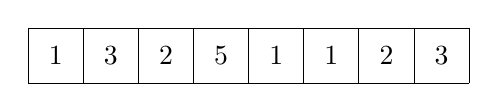
\begin{tikzpicture}[scale=0.7]
\draw (0,0) grid (8,1);

\node at (0.5,0.5) {$1$};
\node at (1.5,0.5) {$3$};
\node at (2.5,0.5) {$2$};
\node at (3.5,0.5) {$5$};
\node at (4.5,0.5) {$1$};
\node at (5.5,0.5) {$1$};
\node at (6.5,0.5) {$2$};
\node at (7.5,0.5) {$3$};
\end{tikzpicture}
\end{center}
қосындысы 8 болатын ішжиымды қатиды:
\begin{center}
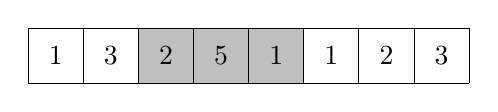
\begin{tikzpicture}[scale=0.7]
\fill[color=lightgray] (2,0) rectangle (5,1);
\draw (0,0) grid (8,1);

\node at (0.5,0.5) {$1$};
\node at (1.5,0.5) {$3$};
\node at (2.5,0.5) {$2$};
\node at (3.5,0.5) {$5$};
\node at (4.5,0.5) {$1$};
\node at (5.5,0.5) {$1$};
\node at (6.5,0.5) {$2$};
\node at (7.5,0.5) {$3$};
\end{tikzpicture}
\end{center}

Есеп шешімін екі нұсқағыш әдісімен $O(n)$ уақытта таба аламыз.
Идеясы -- нұсқағыштарды ішжиымның алғашқы және соңғы мәндеріне сілтеу.
Әр жүрісте сол жақ нұсқағыш бір қадам оңға, ал оң жақ нұсқағыш нәтижесінде
пайда болған ішжиым қосындысы $x$-тен аспайтындай позицияға дейін оңға жылжиды.

% On each turn, the left pointer moves one step
% to the right, and the right pointer moves to the right
% as long as the resulting subarray sum is at most $x$.
Егер қосынды $x$-ке тең болса, шешім табылды.

Үлгі ретінде төмендегі жиым мен мақсатты қосынды $x=8$ болған жағдайды қарастырайық:
\begin{center}
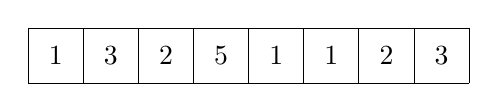
\begin{tikzpicture}[scale=0.7]
\draw (0,0) grid (8,1);

\node at (0.5,0.5) {$1$};
\node at (1.5,0.5) {$3$};
\node at (2.5,0.5) {$2$};
\node at (3.5,0.5) {$5$};
\node at (4.5,0.5) {$1$};
\node at (5.5,0.5) {$1$};
\node at (6.5,0.5) {$2$};
\node at (7.5,0.5) {$3$};
\end{tikzpicture}
\end{center}

Бастапқы ішжиым қосындысы 6 болатын 1, 3 және 2 
мәндерін қамтиды:

\begin{center}
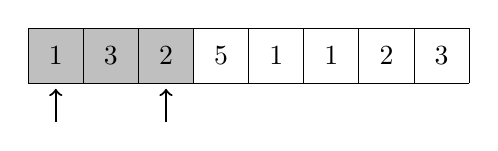
\begin{tikzpicture}[scale=0.7]
\fill[color=lightgray] (0,0) rectangle (3,1);
\draw (0,0) grid (8,1);

\node at (0.5,0.5) {$1$};
\node at (1.5,0.5) {$3$};
\node at (2.5,0.5) {$2$};
\node at (3.5,0.5) {$5$};
\node at (4.5,0.5) {$1$};
\node at (5.5,0.5) {$1$};
\node at (6.5,0.5) {$2$};
\node at (7.5,0.5) {$3$};

\draw[thick,->] (0.5,-0.7) -- (0.5,-0.1);
\draw[thick,->] (2.5,-0.7) -- (2.5,-0.1);
\end{tikzpicture}
\end{center}

Кейін сол жақ нұсқағыш бір қадам оңға жылжиды. Оң жақ нұсқағыш
орнынан қозғалмайды, себебі қозғалған жағдайда ішжиым қосындысы 
$x$-тен асып кетер еді.

\begin{center}
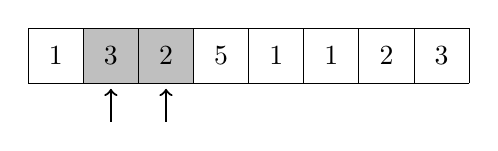
\begin{tikzpicture}[scale=0.7]
\fill[color=lightgray] (1,0) rectangle (3,1);
\draw (0,0) grid (8,1);

\node at (0.5,0.5) {$1$};
\node at (1.5,0.5) {$3$};
\node at (2.5,0.5) {$2$};
\node at (3.5,0.5) {$5$};
\node at (4.5,0.5) {$1$};
\node at (5.5,0.5) {$1$};
\node at (6.5,0.5) {$2$};
\node at (7.5,0.5) {$3$};

\draw[thick,->] (1.5,-0.7) -- (1.5,-0.1);
\draw[thick,->] (2.5,-0.7) -- (2.5,-0.1);
\end{tikzpicture}
\end{center}

Қайтадан сол жақ нұсқағыш бір қадам оңға жылжиды. Осы кезде
оң жақтағы нұсқағыш оңға қарай 3 қадам жасайды. Ішжиым қосындысы -- $2+5+1=8$,
қосындысы $x$ болатын ішжиым табылды.

\begin{center}
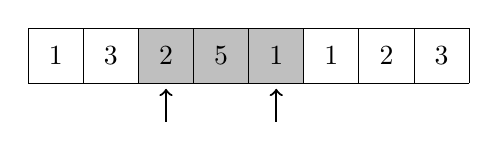
\begin{tikzpicture}[scale=0.7]
\fill[color=lightgray] (2,0) rectangle (5,1);
\draw (0,0) grid (8,1);

\node at (0.5,0.5) {$1$};
\node at (1.5,0.5) {$3$};
\node at (2.5,0.5) {$2$};
\node at (3.5,0.5) {$5$};
\node at (4.5,0.5) {$1$};
\node at (5.5,0.5) {$1$};
\node at (6.5,0.5) {$2$};
\node at (7.5,0.5) {$3$};

\draw[thick,->] (2.5,-0.7) -- (2.5,-0.1);
\draw[thick,->] (4.5,-0.7) -- (4.5,-0.1);
\end{tikzpicture}
\end{center}

Алгоритмнің өңдеу уақыты оң жақ нұсқағыштың жасайтын қадам санына байланысты болады.
Бір итерацияда жасалатын қадамның жоғарғы шегін білмейміз. 
Біз алгоритм барысында нұсқағыштың \emph{жалпылама} $O(n)$ қадам жасайтындағын білеміз,
себебі ол оңға ғана қозғалады.
% we know that the pointer moves \emph{a total of}
% $O(n)$ steps during the algorithm,
% because it only moves to the right.

Алгоритмдегі сол және оң нұсқағыштардың $O(n)$
қадам жасайтындығына байланысты алгоритм $O(n)$ уақытта жұмыс істейді.
% Since both the left and right pointer
% move $O(n)$ steps during the algorithm,
% the algorithm works in $O(n)$ time.

\subsubsection{2SUM есебі}

\index{2SUM есебі}

Екі нұсқағыш тәсілімен шығарылатын тағы бір есептің, яғни 2SUM есебінің шығарылу барысына тоқталайық.  
$n$ саннан тұратын жиым мен $x$ мақсатты сомасы берілген,
қосындылары $x$-ке тең екі жиым мәндерін анықтау немесе мүмкін еместігін хабарлау.

Есепті шығару үшін бірінші жиымды өсу реті бойынша сұрыптаймыз.
Кейін екі нұсқағышты пайдаланып жиымды өтіп шығамыз.
Сол жақ нұсқағыш бірінші мәннен бастап әр жүрісте бір қадам оңға жылжиды.
Оң жақ нұсқағыш соңғы мәннен басталып сол және оң мәндердің қосындысы ең көп дегенде $x$ болғанша
солға жылжиды.
% The right pointer begins at the last value
% and always moves to the left until the sum of the
% left and right value is at most $x$.
Қосынды мәнінің $x$ болуы шешімнің табылғанын білдіреді.

Мысалы, келесі жиым мен мақсатты сома $x=12$ түрінде қарастырайық:
\begin{center}
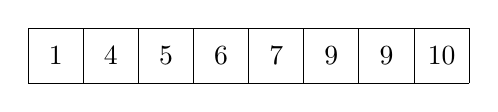
\begin{tikzpicture}[scale=0.7]
\draw (0,0) grid (8,1);

\node at (0.5,0.5) {$1$};
\node at (1.5,0.5) {$4$};
\node at (2.5,0.5) {$5$};
\node at (3.5,0.5) {$6$};
\node at (4.5,0.5) {$7$};
\node at (5.5,0.5) {$9$};
\node at (6.5,0.5) {$9$};
\node at (7.5,0.5) {$10$};
\end{tikzpicture}
\end{center}

Нұсқағыштардың бастапқы позициялары көрсетілгендей.
Мәндер қосындысы -- $1+10=11$, бұл $x$-тен кіші.

\begin{center}
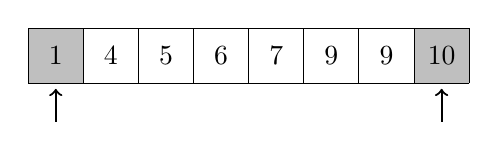
\begin{tikzpicture}[scale=0.7]
\fill[color=lightgray] (0,0) rectangle (1,1);
\fill[color=lightgray] (7,0) rectangle (8,1);
\draw (0,0) grid (8,1);

\node at (0.5,0.5) {$1$};
\node at (1.5,0.5) {$4$};
\node at (2.5,0.5) {$5$};
\node at (3.5,0.5) {$6$};
\node at (4.5,0.5) {$7$};
\node at (5.5,0.5) {$9$};
\node at (6.5,0.5) {$9$};
\node at (7.5,0.5) {$10$};

\draw[thick,->] (0.5,-0.7) -- (0.5,-0.1);
\draw[thick,->] (7.5,-0.7) -- (7.5,-0.1);
\end{tikzpicture}
\end{center}

Кейін сол жақ нұсқағыш бір қадам оңға жылжиды.
Оң жақ нұсқағыш үш қадам солға жылжиды, осылайша 
пайда болған қосынды -- $4+7=11$.

\begin{center}
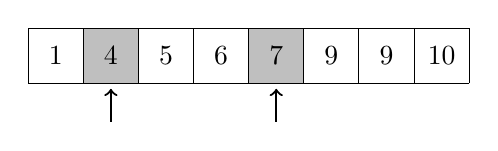
\begin{tikzpicture}[scale=0.7]
\fill[color=lightgray] (1,0) rectangle (2,1);
\fill[color=lightgray] (4,0) rectangle (5,1);
\draw (0,0) grid (8,1);

\node at (0.5,0.5) {$1$};
\node at (1.5,0.5) {$4$};
\node at (2.5,0.5) {$5$};
\node at (3.5,0.5) {$6$};
\node at (4.5,0.5) {$7$};
\node at (5.5,0.5) {$9$};
\node at (6.5,0.5) {$9$};
\node at (7.5,0.5) {$10$};

\draw[thick,->] (1.5,-0.7) -- (1.5,-0.1);
\draw[thick,->] (4.5,-0.7) -- (4.5,-0.1);
\end{tikzpicture}
\end{center}

Бұдан соң сол жақ нұсқағыш қайтадан оңға бір қадам жасайды.
Оң жақ нұсқағыш қозғалмайды, солайша $5+7=12$ шешімі табылды.

\begin{center}
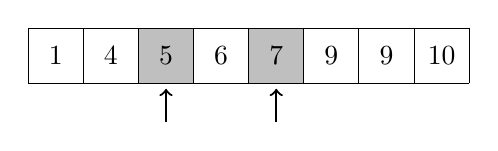
\begin{tikzpicture}[scale=0.7]
\fill[color=lightgray] (2,0) rectangle (3,1);
\fill[color=lightgray] (4,0) rectangle (5,1);
\draw (0,0) grid (8,1);

\node at (0.5,0.5) {$1$};
\node at (1.5,0.5) {$4$};
\node at (2.5,0.5) {$5$};
\node at (3.5,0.5) {$6$};
\node at (4.5,0.5) {$7$};
\node at (5.5,0.5) {$9$};
\node at (6.5,0.5) {$9$};
\node at (7.5,0.5) {$10$};

\draw[thick,->] (2.5,-0.7) -- (2.5,-0.1);
\draw[thick,->] (4.5,-0.7) -- (4.5,-0.1);
\end{tikzpicture}
\end{center}

Алгоритмнің өңдеу уақыты -- $O(n \log n)$, себебі бірінші
жиым $O(n \log n)$ уақыт ішінде сұрыпталып, кейін екі нұсқағыш та 
$O(n)$ қадам жасайды.

Есепті $O(n \log n)$ ішінде бинарлы ізденіс арқылы да шығаруға болатындығын ескеріңіз.
Бұл жағдайда біз жиымды өтіп шығып, әр мән үшін қосынды $x$-ке тең болатындай басқа мән іздейміз.
Ол әрқайсысы $O(\log n)$ уақыт алатын $n$ бинарлы ізденіс арқылы орындала алады.

\index{3SUM есебі}
Қосындысы $x$-ке тең болатын \emph{үш} жиым мәндерін анықтауды 
көздейтін \key{3SUM есебі} алдыңғы қарастырған есепке қарағанда қиынырақ.
Жоғарыда қарастырылған алгоритмді қолдана отырып бұл есепті
$O(n^2)$ уақытта шығара аламыз\footnote{Ұзақ уақыт бойы
3SUM есебін $O(n^2)$ уақытынан тез шешу мүмкін емес деп ойладық.
Бірақ 2014 жылы бұлай еместігі\cite{gro14} анықталды.}.
Қалай шығарылатынын байқадыңыз ба?

\section{Ең жақын кішірек элементтер} %nearest smaller elements

\index{ең жақын кішірек элементтер}

Амортиазцияланған талдау деректер құрылымындағы
операциялар санына баға беру үшін жиі қолданылады.
Операциялар бірқалыпсыз, алгоритмнің белгілі бір бөлігінде
жиірек орындалатындай болып таратылуы мүмкін.
Дегенмен операциялар саны шектеулі болмақ.
% The operations may be distributed unevenly so
% that most operations occur during a
% certain phase of the algorithm, but the total
% number of the operations is limited.

Үлгі ретінде жиымдағы әр элемент үшін \key{ең жақын кішірек элементті},
яки ең бірінші болып сол элементке дейін кездесетін кішірек элементті анықтайтын
есепті қарастырайық.
Ондай элемент болмаған жағдайда алгоритм
жоқ екенін хабарлауы қажет. 
Енді есепті стэк құрылымын пайдалану арқылы қалай тиімді шешуге болатынын көреміз.

Біз жиым элементтерінің стегін сақтай отырып, жиымды солдан оңға қарай аралаймыз.
%We go through the array from left to right
%and maintain a stack of array elements.
Әр қадам сайын біз төбедегі элемент ағымдағы элементтен кіші болып шыққанға дейін немесе стек босап қалғанға дейін стэктен элементтерді өшіріп отырамыз. Осыдан кейін біз стэктің төбесіндегі элемент - ағымдағы ең жақын кіші элемент екенін немесе стэк бос 
болған жағдайда, ондай элементтің жоқтығын хабарлаймыз.
Соңында ағымдағы элементті стэкке қосамыз.

Мысал ретінде келесі жиымды қарастырайық: 
\begin{center}
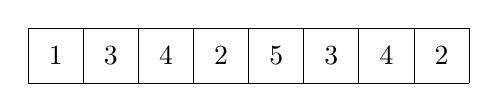
\begin{tikzpicture}[scale=0.7]
\draw (0,0) grid (8,1);

\node at (0.5,0.5) {$1$};
\node at (1.5,0.5) {$3$};
\node at (2.5,0.5) {$4$};
\node at (3.5,0.5) {$2$};
\node at (4.5,0.5) {$5$};
\node at (5.5,0.5) {$3$};
\node at (6.5,0.5) {$4$};
\node at (7.5,0.5) {$2$};
\end{tikzpicture}
\end{center}

Бірінші 1, 3 және 4 сандары стэкке қосылады, себебі әр элемент алдыңғысынан үлкенірек.
Сол себепті 4 үшін ең жақын кішірек элемент -- 3, ал 3 үшін ең жақын кішірек элемент 2 болмақ.
\begin{center}
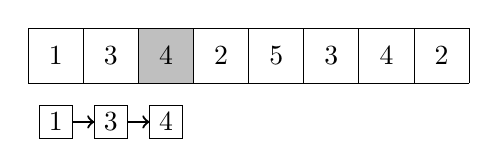
\begin{tikzpicture}[scale=0.7]
\fill[color=lightgray] (2,0) rectangle (3,1);
\draw (0,0) grid (8,1);

\node at (0.5,0.5) {$1$};
\node at (1.5,0.5) {$3$};
\node at (2.5,0.5) {$4$};
\node at (3.5,0.5) {$2$};
\node at (4.5,0.5) {$5$};
\node at (5.5,0.5) {$3$};
\node at (6.5,0.5) {$4$};
\node at (7.5,0.5) {$2$};

\draw (0.2,0.2-1.2) rectangle (0.8,0.8-1.2);
\draw (1.2,0.2-1.2) rectangle (1.8,0.8-1.2);
\draw (2.2,0.2-1.2) rectangle (2.8,0.8-1.2);

\node at (0.5,0.5-1.2) {$1$};
\node at (1.5,0.5-1.2) {$3$};
\node at (2.5,0.5-1.2) {$4$};

\draw[->,thick] (0.8,0.5-1.2) -- (1.2,0.5-1.2);
\draw[->,thick] (1.8,0.5-1.2) -- (2.2,0.5-1.2);
\end{tikzpicture}
\end{center}

Келесі элемент -- 2. Ол стэктің жоғарысындағы екі элементтен кіші.
Сол себепті 3 пен 4 элементтері стэктен өшіріліп, 2 стэкке қосылады.
Оның ең жақын кішірек элементі -- 1:
\begin{center}
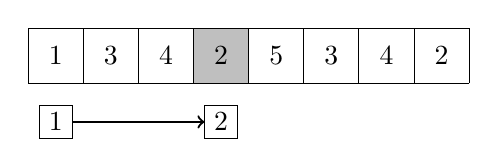
\begin{tikzpicture}[scale=0.7]
\fill[color=lightgray] (3,0) rectangle (4,1);
\draw (0,0) grid (8,1);

\node at (0.5,0.5) {$1$};
\node at (1.5,0.5) {$3$};
\node at (2.5,0.5) {$4$};
\node at (3.5,0.5) {$2$};
\node at (4.5,0.5) {$5$};
\node at (5.5,0.5) {$3$};
\node at (6.5,0.5) {$4$};
\node at (7.5,0.5) {$2$};

\draw (0.2,0.2-1.2) rectangle (0.8,0.8-1.2);
\draw (3.2,0.2-1.2) rectangle (3.8,0.8-1.2);

\node at (0.5,0.5-1.2) {$1$};
\node at (3.5,0.5-1.2) {$2$};

\draw[->,thick] (0.8,0.5-1.2) -- (3.2,0.5-1.2);
\end{tikzpicture}
\end{center}

Кейін 5 элементі 2-ден үлкенірек болғандықтан
осы стэкке қосылып, оның ең жақын кішірек элементі 2 болады:
\begin{center}
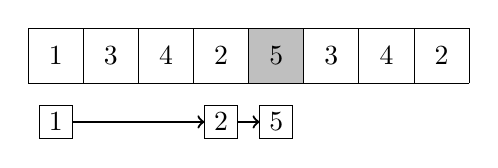
\begin{tikzpicture}[scale=0.7]
\fill[color=lightgray] (4,0) rectangle (5,1);
\draw (0,0) grid (8,1);

\node at (0.5,0.5) {$1$};
\node at (1.5,0.5) {$3$};
\node at (2.5,0.5) {$4$};
\node at (3.5,0.5) {$2$};
\node at (4.5,0.5) {$5$};
\node at (5.5,0.5) {$3$};
\node at (6.5,0.5) {$4$};
\node at (7.5,0.5) {$2$};

\draw (0.2,0.2-1.2) rectangle (0.8,0.8-1.2);
\draw (3.2,0.2-1.2) rectangle (3.8,0.8-1.2);
\draw (4.2,0.2-1.2) rectangle (4.8,0.8-1.2);

\node at (0.5,0.5-1.2) {$1$};
\node at (3.5,0.5-1.2) {$2$};
\node at (4.5,0.5-1.2) {$5$};

\draw[->,thick] (0.8,0.5-1.2) -- (3.2,0.5-1.2);
\draw[->,thick] (3.8,0.5-1.2) -- (4.2,0.5-1.2);
\end{tikzpicture}
\end{center}

Бұдан соң 5 элементі стэктен өшіріліп, стэкке 3 пен 4 элементтері қосылады:
\begin{center}
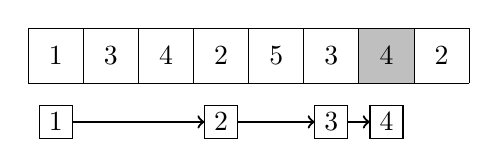
\begin{tikzpicture}[scale=0.7]
\fill[color=lightgray] (6,0) rectangle (7,1);
\draw (0,0) grid (8,1);

\node at (0.5,0.5) {$1$};
\node at (1.5,0.5) {$3$};
\node at (2.5,0.5) {$4$};
\node at (3.5,0.5) {$2$};
\node at (4.5,0.5) {$5$};
\node at (5.5,0.5) {$3$};
\node at (6.5,0.5) {$4$};
\node at (7.5,0.5) {$2$};

\draw (0.2,0.2-1.2) rectangle (0.8,0.8-1.2);
\draw (3.2,0.2-1.2) rectangle (3.8,0.8-1.2);
\draw (5.2,0.2-1.2) rectangle (5.8,0.8-1.2);
\draw (6.2,0.2-1.2) rectangle (6.8,0.8-1.2);

\node at (0.5,0.5-1.2) {$1$};
\node at (3.5,0.5-1.2) {$2$};
\node at (5.5,0.5-1.2) {$3$};
\node at (6.5,0.5-1.2) {$4$};

\draw[->,thick] (0.8,0.5-1.2) -- (3.2,0.5-1.2);
\draw[->,thick] (3.8,0.5-1.2) -- (5.2,0.5-1.2);
\draw[->,thick] (5.8,0.5-1.2) -- (6.2,0.5-1.2);
\end{tikzpicture}
\end{center}

Ақырында 1-ден өзге барлық элементтер өшіріліп, соңғы 2 элементі стэкке қосылады:

\begin{center}
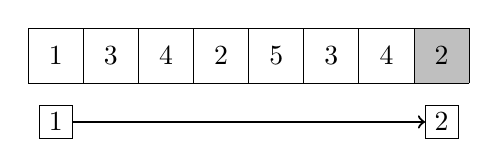
\begin{tikzpicture}[scale=0.7]
\fill[color=lightgray] (7,0) rectangle (8,1);
\draw (0,0) grid (8,1);

\node at (0.5,0.5) {$1$};
\node at (1.5,0.5) {$3$};
\node at (2.5,0.5) {$4$};
\node at (3.5,0.5) {$2$};
\node at (4.5,0.5) {$5$};
\node at (5.5,0.5) {$3$};
\node at (6.5,0.5) {$4$};
\node at (7.5,0.5) {$2$};

\draw (0.2,0.2-1.2) rectangle (0.8,0.8-1.2);
\draw (7.2,0.2-1.2) rectangle (7.8,0.8-1.2);

\node at (0.5,0.5-1.2) {$1$};
\node at (7.5,0.5-1.2) {$2$};

\draw[->,thick] (0.8,0.5-1.2) -- (7.2,0.5-1.2);
\end{tikzpicture}
\end{center}

Алгоритмнің тиімділігі стэк операцияларының жалпы санына тәуелді.
Егер алынған элемент стэктің жоғарғы элементінен үлкен болса,
ол стэкке бірден тиімді қосылады.
Бірақ кейде стэк бірнеше үлкенірек элементтерді қамтуы мүмкін
және оларды өшіру уақытты алады. Дегенмен әр элемент стэкке \emph{бір рет қана қосылады}
және өшірілуі \emph{көп дегенде бір рет} орын алады.
Сондықтан әр элемент $O(1)$ стэк операцияларын тудырып, алгоритм $O(n)$ уақытында орындалады.

\section{Жылжымалы терезе минимумы}

\index{жылжымалы терезе}
\index{жылжымалы терезе минимумы}

\key{Жылжымалы терезе} -- константалы-өлшемді ішжиым,
ол жиым бойымен солдан оңға қарай жылжиды.
Әр терезе позициясында терезе ішіндегі элементтер туралы
қандай да бір ақпаратты анықтағымыз келеді. Бұл бөлікте 
\key{жылжымалы терезе минимумы} есебіне назар аударамыз.
Мұнда әр терезе ішіндегі ең кіші мәнді хабарлауымыз қажет.

Жылжымалы терезелердегі минимумдарды есептеу үшін ең жақын кішірек элементтерді табу барысындағы идеяны қолдануға болады.  
Бірақ бұл жолы бізге әр элементі алдыңғысынан 
үлкенірек, ал бірінші элементі әрдайым терезенің ішіндегі ең аз элементке сәйкес келетін кезек қажет болады. 
Әр терезе қозғалысы сайын кезек соңынан 
элементтерді алып отырамыз, бұл кезектің соңғы саны терезенің жаңа элементінен кіші 
болғанша немесе кезек босағанша жалғасады. Сонымен қатар егер кезектің алғашқы элементі терезеде болмаса,
оны өшіреміз. Соңында терезенің жаңа элементін кезек соңына қосамыз.

Мысал ретінде келесі жиымды қарастырайық:

\begin{center}
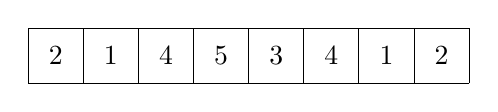
\begin{tikzpicture}[scale=0.7]
\draw (0,0) grid (8,1);

\node at (0.5,0.5) {$2$};
\node at (1.5,0.5) {$1$};
\node at (2.5,0.5) {$4$};
\node at (3.5,0.5) {$5$};
\node at (4.5,0.5) {$3$};
\node at (5.5,0.5) {$4$};
\node at (6.5,0.5) {$1$};
\node at (7.5,0.5) {$2$};
\end{tikzpicture}
\end{center}

Жылжымалы терезе өлшемін 4 деп алайық. Терезенің бірінші позициясында
ең кіші мән -- 1:
\begin{center}
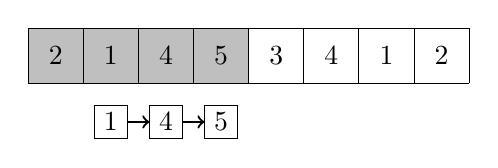
\begin{tikzpicture}[scale=0.7]
\fill[color=lightgray]
(0,0) rectangle (4,1);
\draw (0,0) grid (8,1);

\node at (0.5,0.5) {$2$};
\node at (1.5,0.5) {$1$};
\node at (2.5,0.5) {$4$};
\node at (3.5,0.5) {$5$};
\node at (4.5,0.5) {$3$};
\node at (5.5,0.5) {$4$};
\node at (6.5,0.5) {$1$};
\node at (7.5,0.5) {$2$};

\draw (1.2,0.2-1.2) rectangle (1.8,0.8-1.2);
\draw (2.2,0.2-1.2) rectangle (2.8,0.8-1.2);
\draw (3.2,0.2-1.2) rectangle (3.8,0.8-1.2);

\node at (1.5,0.5-1.2) {$1$};
\node at (2.5,0.5-1.2) {$4$};
\node at (3.5,0.5-1.2) {$5$};

\draw[->,thick] (1.8,0.5-1.2) -- (2.2,0.5-1.2);
\draw[->,thick] (2.8,0.5-1.2) -- (3.2,0.5-1.2);
\end{tikzpicture}
\end{center}

Кейін терезе бір қадам оңға жылжиды.
Жаңа элемент 3 кезектегі 4 пен 5 элементтерінен кішірек,
сондықтан 4 пен 5 элементтері кезектен өшіріліп,
3 қосылды. Ең кіші элемент әлі де 1 бола береді.
\begin{center}
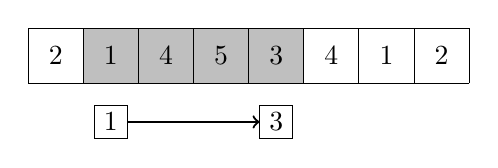
\begin{tikzpicture}[scale=0.7]
\fill[color=lightgray] (1,0) rectangle (5,1);
\draw (0,0) grid (8,1);

\node at (0.5,0.5) {$2$};
\node at (1.5,0.5) {$1$};
\node at (2.5,0.5) {$4$};
\node at (3.5,0.5) {$5$};
\node at (4.5,0.5) {$3$};
\node at (5.5,0.5) {$4$};
\node at (6.5,0.5) {$1$};
\node at (7.5,0.5) {$2$};

\draw (1.2,0.2-1.2) rectangle (1.8,0.8-1.2);
\draw (4.2,0.2-1.2) rectangle (4.8,0.8-1.2);

\node at (1.5,0.5-1.2) {$1$};
\node at (4.5,0.5-1.2) {$3$};

\draw[->,thick] (1.8,0.5-1.2) -- (4.2,0.5-1.2);
\end{tikzpicture}
\end{center}

Бұдан соң терезе тағы жылжиды,
енді ең кіші элемент 1 терзеге кірмейді.
Сондықтан ол кезектен өшіріліп, ең кіші мән 3-ке теңеседі.
Сонымен қатар жаңа элемент 4 кезекке қосылады.
\begin{center}
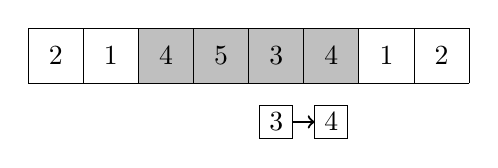
\begin{tikzpicture}[scale=0.7]
\fill[color=lightgray] (2,0) rectangle (6,1);
\draw (0,0) grid (8,1);

\node at (0.5,0.5) {$2$};
\node at (1.5,0.5) {$1$};
\node at (2.5,0.5) {$4$};
\node at (3.5,0.5) {$5$};
\node at (4.5,0.5) {$3$};
\node at (5.5,0.5) {$4$};
\node at (6.5,0.5) {$1$};
\node at (7.5,0.5) {$2$};

\draw (4.2,0.2-1.2) rectangle (4.8,0.8-1.2);
\draw (5.2,0.2-1.2) rectangle (5.8,0.8-1.2);

\node at (4.5,0.5-1.2) {$3$};
\node at (5.5,0.5-1.2) {$4$};

\draw[->,thick] (4.8,0.5-1.2) -- (5.2,0.5-1.2);
\end{tikzpicture}
\end{center}

Келесі жаңа элемент 1 кезектегі барлық элементтерден кіші.
Сол себепті барлық элементтер өшіріліп, кезек енді тек 1 элементін қамтиды:
\begin{center}
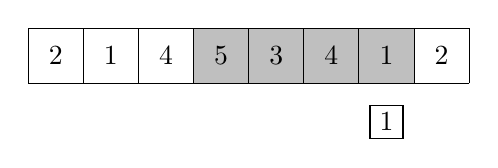
\begin{tikzpicture}[scale=0.7]
\fill[color=lightgray] (3,0) rectangle (7,1);
\draw (0,0) grid (8,1);

\node at (0.5,0.5) {$2$};
\node at (1.5,0.5) {$1$};
\node at (2.5,0.5) {$4$};
\node at (3.5,0.5) {$5$};
\node at (4.5,0.5) {$3$};
\node at (5.5,0.5) {$4$};
\node at (6.5,0.5) {$1$};
\node at (7.5,0.5) {$2$};

\draw (6.2,0.2-1.2) rectangle (6.8,0.8-1.2);

\node at (6.5,0.5-1.2) {$1$};
\end{tikzpicture}
\end{center}

Ақырында терезе өзінің соңғы позициясына жетеді.
2 элементі кезекке қосылады, бірақ терезедегі ең кіші элемент 1 болып қала береді.
\begin{center}
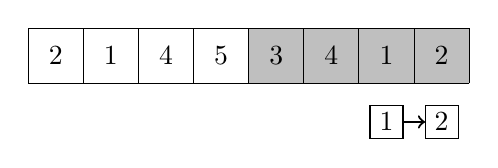
\begin{tikzpicture}[scale=0.7]
\fill[color=lightgray] (4,0) rectangle (8,1);
\draw (0,0) grid (8,1);

\node at (0.5,0.5) {$2$};
\node at (1.5,0.5) {$1$};
\node at (2.5,0.5) {$4$};
\node at (3.5,0.5) {$5$};
\node at (4.5,0.5) {$3$};
\node at (5.5,0.5) {$4$};
\node at (6.5,0.5) {$1$};
\node at (7.5,0.5) {$2$};

\draw (6.2,0.2-1.2) rectangle (6.8,0.8-1.2);
\draw (7.2,0.2-1.2) rectangle (7.8,0.8-1.2);

\node at (6.5,0.5-1.2) {$1$};
\node at (7.5,0.5-1.2) {$2$};

\draw[->,thick] (6.8,0.5-1.2) -- (7.2,0.5-1.2);
\end{tikzpicture}
\end{center}

Жиымның әр элементі кезекке тек бір рет қосылғандықтан 
және кезектен көп дегенде бір-ақ рет өшірілгендіктен,
алгоритм $O(n)$ уақытта жұмыс жасайды.